\chapter{Il Magnetismo Stazionario}

Andremo in questo capitolo, in modo analogo a quanto fatto con l'elettricità, a osservare i campi magnetici in condizioni \textit{statiche}. 

\section{Introduzione alla Magnetostatica}

\subsection{Fatti Sperimentali}
Possiamo osservare che alcuni materiali palesano l'esistenza di una \textbf{nuova forza} non descrivibile tramite le teorie fino a questo punto note. Questa forza può essere \textit{attrattiva} o \textit{repulsiva} ed è localizzata ai \textbf{poli del materiale}. 

Prendendo un materiale molto piccolo tale da non perturbare il nostro sistema, chiamato \textbf{ago magnetico}, osserviamo che tale oggetto si \textbf{orienta} sempre in una stessa direzione. Questo ci dice che esiste un \textit{effetto magnetico} dovuto al pianeta Terra. 

Nel momento in cui \textit{speziamo una calamita} possiamo osservare che non è possibile isolare il polo nord dal polo sud, troveremo di nuovo due pezzi di calamita dotati ciasuno di un polo nord e di un polo sud. Questo ci dice che \textbf{non esiste il monopolo magnetico}.

Un altro esperimento molto importante che possiamo fare è fatto considerando un filo di corrente che attraversa una lastra cosparsa di aghi magnetici, possiamo osservare che gli aghi si orientano secondo delle \textbf{linee chiuse attorno al filo}. In pratica la corrente elettrica è causa di \textit{effetti magnetici}.

Concludiamo che la sorgente del campo magnetico $\vec{B}$ è la corrente elettrica, ma le correnti sono cariche in moto, quindi ci aspetteremo di avere come campo magnetico prodotto dalla carica microscopica in moto. 

Abbiamo dunque scoperto l'esistenza di un \textbf{campo magnetico} ch va ad agire sugli oggetti attorno ad esso. Così come il campo elettrostatico agisce sulle cariche con una forza data da $qE$ ed è generato da una sorgente di cariche, per il campo magnetico avremo che le sorgenti sono le \textbf{cariche in moto} e che gli oggetti su cui agisce sono sempre cariche in moto e le correnti.

\section{Forza di Lorentz}
Poniamo di avere un campo magnetico e consideriamo un oggetto su cui tale campo agisce (una carica in moto). Potremo osservare che l'intensità della forza è proporzionale alla carica, alla velocità e al campo magnetico. Mentre in elettrostatica abbiamo che la forza è parallela al campo, nel magnetismo parallelamente al campo la forza è nulla, così parallelamente alla velocità. Osserviamo che questa nuova forza è \textbf{perpendicolare} al campo $B$ e alla velocità. 

\begin{figure}[th]
	\centering
	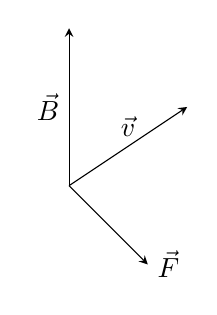
\begin{tikzpicture}
		\draw[-stealth] (0,0) -- (0,2) node [midway, left] {$\vec{B}$} ;
		\draw [-stealth] (0,0) -- (1.5,1) node [midway, above] {$\vec{v}$};
		\draw[-stealth] (0,0) -- (1, -1) node [right]{$\vec{F}$};
	\end{tikzpicture}
	\caption{Forza di Lorentz}
\end{figure}

Dunque avremo che la forza di Lorentz sarà espressa da 

\begin{large}
	\begin{equation} \label{eq:forza_lorentz}
		\vec{F}_{Lorentz} = q \vec{v} \times \vec{B}
	\end{equation}
\end{large}

Ipotizziamo di ingrandire un filo conduttore di sezione $s$ e di lunghezza $dl$. Al suo interno avremo delle cariche in moto. Su ognuna di queste cariche agirà chiaramente una forza di Lorentz. Andrò a contare ognuna di queste cariche mettendo le forze in una sommatoria. Ricordo inoltre che la densità di corrente $\vec{j}$ è data dal numero dei portatori di carica, per la carica e la velocità di deriva: $j = Nqv$ e che l'intensità $i = \vec{j} \cdot d\vec{S}$. 

Troveremo dunque che la risultante delle forze di Lorentz che agiscono in un conduttore è esprimibile in termini di intensità di corrente:

\begin{large}
	\begin{equation}
		d\vec{F} = idl \times B
	\end{equation}
\end{large}

Quella descritta in questa equazione è detta \textbf{2° Legge di Laplace}. Chiaramente, dato che la forza magnetica è ortogonale alla velocità e al campo magnetico, non avremo lavoro, dunque non avremo un potenziale scalare. In sostanza, anche ricordando il fatto che non esiste una sorgente isolata di carica magnetica, le \textbf{linee di campo} del campo magnetico sono \textbf{chiuse}. Potremo quindi trovare la seguente equazione importantissima:

\begin{tcolorbox}[colframe=red, colback=red!10, title=1° Equazione di Maxwell nel Magnetismo Stazionario]
	\begin{large}
		\begin{equation}
			\Phi(\vec{B}) = 0
		\end{equation}
	\end{large}
\end{tcolorbox}

\section{Dipolo Magnetico in campo esterno $\vec{B}$ }
Definiamo \textbf{dipolo magnetico} una spira elementare, ovvero della quale non ci importa la geometria, percorsa da una corrente $i$. Attraverso questo concetto andiamo a definire il concetto di \textbf{momento di dipolo}: 

\begin{large}
	\begin{equation} \label{eq_momento_dipolo_magnetico}
		\vec{\mu} \coloneqq i\vec{S} \;\; \left[Am^2\right]
	\end{equation}
\end{large}

Consideriamo ora la nostra spira percorsa da corrente $i$ immersa in un campo magnetico stazionario $\vec{B}$. 

\begin{figure}[ht]
	\centering
	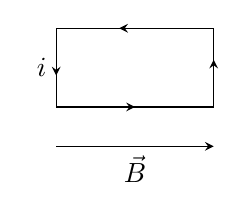
\begin{tikzpicture}
		\draw (0,0) -- (2,0) -- (2,1) -- (0,1) -- (0,0) node [midway, left] {$i$};
		\draw [-stealth] (0.8,0) -- (1, 0);
		\draw [-stealth] (2,0.4) -- (2,0.6);
		\draw [-stealth] (1,1) -- (0.8,1);
		\draw [-stealth] (0,0.6) -- (0,0.4);
		\draw [-stealth] (0,-0.5) -- (2,-0.5) node [midway, below] {$\vec{B}$};
	\end{tikzpicture}
\end{figure}

Chiameremo il lato lungo $b$ e il lato corto $a$, e, ricordando la formulazione della Forza di Lorentz $F = idl \times B$,  avremo sui lati $a$ una forza data da $F = iaB$, mentre sui lati $b$ avremo forza nulla. Chiaramente le due forze saranno in contrapposizione, dunque il nostro oggetto non traslerà ma avrà un momento torcente non nullo, con $\tau = (r \times F) = iabB$, in particolare avremo che 

$$\vec{\tau} = \vec{\mu} \times \vec{B} $$

ovvero il momento \textbf{meccanico} di un dipolo magnetico o di una spira immersa in un campo esterno B. Avremo anche che l'\textbf{energia} nel dipolo immerso nel campo esterno sarà data da: 

\begin{equation}
	U = -\vec{\mu} \cdot \vec{B}
\end{equation}

Si noti l'analogia con la formulazione dell'energia immagazzinata nel dipolo elettrico.

\section{Teorema di Ampere}
Andiamo ora a vedere lo strumento che ci consentirà di calcolare il campo magnetico in condizioni stazionarie. Abbiamo visto che il lavoro della forza magnetica è sempre nullo, dunque non ci sarà possibile trovare un potenziale magnetico. Per questo motivo ci possiamo aspettare che lungo un percorso chiuso non avremo circuitazione di campo nulla. 

Questo teorema ci permetterà di ricavare il campo nello spazio a partire dalle \textbf{cariche in moto}, ovvero le sorgenti. In sostanza, contrariamente a quanto visto nella forza di Lorentz, andiamo ad indagare come le cariche in moto agiscono sul campo magnetico (la forza di Lorentz ci dice come le cariche in modo immerse in un campo interagiscano con questo). 

Si consideri un filo percorso da una corrente $\vec{i}$ e guardiamo le linee di campo generate da tale corrente, potremo osservare delle circonferenze concentriche che si avvolgono attorno a tale filo (lungo tutto il filo). 

\begin{figure}[th]
	\centering
	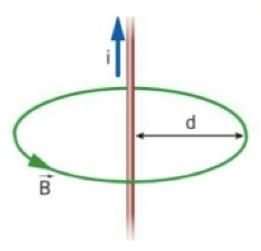
\includegraphics[width=0.5\linewidth]{Media/linee_campo_B}
	\caption{Linee di Campo Magnetico}
	\label{fig:lineecampob}
\end{figure}

Notiamo che poteva andare soltanto in questo modo, infatti se consideriamo un filo sufficientemente lungo da trasformare gli effetti ai bordi, abbiamo simmetria cilindrica, avendo delle linee chiuse, saranno per forza delle circonferenze. Poiché le linee sono delle circonferenza, il campo sarà costante in tutte le circonferenze distanti $r$ dal nostro filo ($\vec{B}$ andrà giù al massimo come $r^{-1}$ e osserviamo che $\vec{B}$ è \textbf{proporzionale} alle correnti. 

$$
\begin{cases}
|B| \propto i \\
|B| \propto \frac{1}{r}
\end{cases}
$$

Tramite queste osservazioni possiamo formulare il nostro \textbf{teorema di Ampere}

\begin{tcolorbox}[colframe=red, colback=red!10, title=1° Equazione di Maxwell nel Magnetismo Stazionario]
	\begin{large}
		\begin{equation}
			\oint_\Gamma \vec{B} \cdot d\vec{l} = \mu_0 i_{concat.}
		\end{equation}
	\end{large}
\end{tcolorbox}

Ovvero il la circuitazione del campo magnetico lungo una \textit{qualsiasi linea chiusa} è dato dalla \textbf{permeabilità magnetica} moltiplicata per le \textbf{correnti concatenate} a tale linea chiusa.

Sappiamo che la carica in moto è una corrente, possiamo quindi utilizzare Lorentz, ma avremo anche qualcosa che riguarda Laplace.In particolare la forza di Laplace che agisce su un elemento di filo immerso in un campo $\vec{B}$ è data da $F = idl \times B$. 

\section{Azione Meccanica tra Correnti}
Siamo in una situazione in cui abbiamo un filo percorso da $i_1$ con, a una certa distanza $d$, un altro filo percorso da $i_2$. Ci chiediamo quale sia la forza agente sui due fili, utilizzeremo questo risultati per andare a definire l'unita di misura dell'\textbf{Ampere}. 


Avremo che $i_1$ produrrà un campo $B_1$ che andrà ad agire in tutto lo spazio circostante, e la stessa cosa farà $i_2$ producendo $B_2$. In sostanza avremo che sulla corrente $i_2$ agirà la forza seguente: 

$$
dF_{1\rightarrow2} = i_2 d\vec{l} \times \vec{B}_1(r=d)
$$

Sappiamo che $B_1 = \mu_0i/2\pi r $, avremo dunque: 

$$ 
dF = i_2 \frac{\mu_0 i_1}{2\pi d}
$$

Tale forza sarà \textbf{attrattiva} e si registrerà in ugual misura con pedici invertiti.  Da ciò ricaviamo che correnti \textbf{parallele} si \textbf{attraggono} e che correnti \textbf{antiparallele} si \textbf{respingono}.

\section{Flusso del Campo Magnetico B}
In questo paragrafo siamo interessati, dato un campo magnetico $\vec{B}$ e una superficie $sup$ a calcolare il flusso $\int_{sup} B(r) \cdot dS$, tale superficie sarà chiaramente \textbf{aperta}, in quanto le linee di campo sono chiuse. 

Prima di andare a chiarire questo calcolo andiamo a introdurre due concetti che sono la \textbf{mutua induzione} e l'\textbf{autoinduzione}. 

\subsection{Mutua Induzione}

Si considerino due circuiti $\Gamma_1, \Gamma_2$,  il circuito $\Gamma_1$ percorso da una $i_1$,  produrrà un campo magnetico $B_1$ che sarà percepito anche nel circuito $\Gamma_2$. Andiamo ora a modellare il flusso del campo magnetico $B_1$ sul circuito $\Gamma_2$, più precisamente sarà il \textbf{flusso di} $B_1$ \textbf{concatenato al circuito} $\Gamma_2$. 

\begin{large}
	\begin{equation}
		\Phi_{1\rightarrow2}  = \int_{\Sigma_2} B_1 \cdot dS = M_{12}i_1
	\end{equation}
\end{large}

tale coefficiente $M$ è detto \textbf{coefficiente di mutua induzione} che è uguale al coefficiente di mutua induzione di 2 su 1 e dipende soltanto da \textit{fattori geometrici} relativi ai due circuiti presi in considerazione, dunque analogamente avremo che il flusso di 2 su 1 sarà: 

$$
\Phi_{2\rightarrow1} = Mi_2
$$

\subsection{Autoinduzione}
Sappiamo che la corrente che percorre un circuito produce un campo che va ad avvolgersi attorno al circuito stesso, potremo in pratica osservare per un circuito isolato un \textbf{autoflusso} sulla superficie del circuito preso in considerazione. Più precisamente andremo a parlare di un \textbf{autoflusso concatenato}

\begin{large}
	\begin{equation}
		\Phi = \int_{\Sigma} B\cdot dS = Li
	\end{equation}
\end{large}

dove $L$ è detto \textbf{coefficiente di autoinduzione}, o \textbf{induttanza} che si misura in Henry $\left[H\right]$.

\section{1° Legge Elementare di Laplace}
Dopo aver visto quali siano le sorgenti dei campi (le correnti) ed aver visto come il campo vada ad agire su correnti immerse in questo campo, esercitando \textbf{Forza di Lorentz e di Laplace}, vogliamo, analogamente a quanto visto in elettrostatica, vedere quale sia il \textbf{campo elementare} prodotto da una \textbf{corrente unitaria}. 

In elettrostatica abbiamo infatti che un volumetto di cariche $dq$ produce un campo elementare
$$
d\vec{E} = \frac{dq}{4\pi\epsilon_0r^2}\hat{r}
$$

Quindi dato un elemento $dl$ percorso da una corrente $i$, avremo che questo produce un campo magnetico elementare espresso da 

\begin{large}
\begin{equation} \label{eq_campoElementare}
		d\vec{B} = \frac{\mu_0}{4\pi} i \frac{d\vec{l} \times \vec{r}}{r^2}
\end{equation}
\end{large}

Utilizzando il fatto che $i = j Sup$ e che $j = nq<v>$ e l'equazione di cui sopra, potremo ricavare il \textbf{campo magnetico di una singola carica in moto}

\begin{large}
	\begin{equation}
		\vec{B}_q = \frac{\mu_0}{4\pi} q\vec{v} \times \frac{\hat{r}}{r^2}
	\end{equation}
\end{large}

Questo indica che nel momento in cui abbiamo una \textit{singola carica in moto}, questa genera \textbf{campo magnetico}. 

\section{Energia del Campo Magnetico}
Abbiamo visto che nel caso di campo elettrostatico, andando a considerare un volumetto $d\tau$ abbiamo una densità di energia $\mu_E = E^2 \epsilon_0 / 2$. Vogliamo ora indagare la densità di energia relativa al campo magnetico. 

Sia $\vec{B}$ un campo magnetico \textit{qualunque} in una regione di spazio, in tale regione avremo una \textbf{densità di energia} data da un'equazione molto simile a quella vista in elettrostatica; questo avviene per il fatto che ci sia una strettissima analogia tra magnetismo e elettrostatica. 

\begin{large}
	\begin{equation}\label{eq_densita_energia_campo_magnetico}
		\mu_B = \frac{1}{2\mu_0} B^2
	\end{equation}
\end{large}

Il valore di tale densità, sarà chiaramente dato da $J/m^3$. Per calcolare l'energia immagazzinata in un sistema quindi, considereremo il campo magnetico, ne calcoleremo la densità e andremo ad integrare tale densità nel nostro sistema.